% Das Management Summary richtet sich in der Praxis an die "Chefs des Chefs", d.
% h. an die Vorgesetzten des Auftraggebers (diese sind in der Regel keine
% Fachspezialisten).
% Die Sprache soll knapp, klar und stark untergliedert sein.
% Zu verwenden ist folgenden Gliederung:
% - Ausgangslage - Vorgehen, Technologien - Ergebnisse - Ausblick (optional)

\chapter*{Management Summary}\addcontentsline{toc}{chapter}{Management Summary}

\paragraph{Ausgangslage}~\\
In der Verkehrs- und Raumplanung werden ÖV-Güteklassen für die Beurteilung eines Standortes bezüglich der Erschliessung mit dem öffentlichen Verkehr verwendet.
Durch diese können Entscheidungen betreffend der Standortentwicklung getroffen werden.
Die gängige Strategie sieht vor, an bereits gut erschlossenen Standorten zu verdichten statt neues Bauland zu erschliessen, um nachträglich die ÖV-Infrastruktur hochziehen zu müssen.
Der Nutzen der ÖV-Güteklassen beschränkt sich nicht auf Verkehrs- und Raumplaner.
Privatpersonen können ebenso bei der Wohnungs- wie auch der Jobsuche davon Gebrauch machen.
Ein Wohnort mit guter ÖV-Anbindung ist in Zeiten erhöhter Mobilität von hohem Stellenwert.

Die Methodik zur Erhebung von ÖV-Güteklassen wurde erstmals 1993 in einer inzwischen ersetzten Schweizer Norm festgelegt.
Auf Grundlagen dieser hat das Bundesamt für Raumentwicklung (ARE) sowie verschiedene Kantone Berechnungsmethodiken entwickelt.
Diese weichen unterschiedlich stark von der Norm ab.

Diese Berechnungsmethodiken sind für die heutigen technischen Möglichkeiten überholt.
So wird unteranderem das Einzugsgebiet wie in Abbildung \ref{fig:air_line_ARE} sichtbar mit Luftlinien berechnet. 

\begin{figure}[ht]
    \centering
    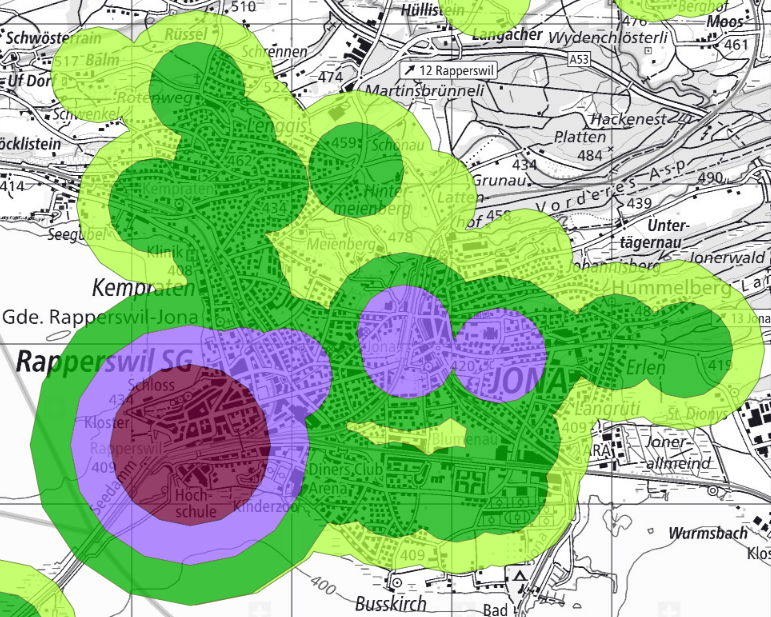
\includegraphics[width=0.50\linewidth]{start/img/air_line_ARE.png}
    \caption[Luftlinie bei Einzugsgebieten]{Luftlinie bei Einzugsgebieten~\cite{berechnung_are}}
    \label{fig:air_line_ARE}
\end{figure}

Der Wegführung wird in den aktuellen Lösungen keine und der Topographie nur wage Beachtung geschenkt.
So ist nicht klar, in welchem Mass eine anspruchsvolle Topographie zu Buche schlägt, denn eine Haltestelle in einem steilen Gebiet hat ein geringeres Einzugsgebiet als eine Haltestellen in einem flachen Gelände.

Erfahrungen aus der Praxis haben gezeigt, dass die bestehenden Lösungen einige Tücken in der Berechnung der Güteklassen aufweisen, welche zu einem falschen Schluss führen können.

\paragraph{Ziele, Vorgehen und Technologien}~\\
Im Kontext der Arbeit ÖV-Güteklassen 2018 wird in einem ersten Schritt eine neue Spezifikation entwickelt, welche auf dem Fundament der bestehenden Lösungen aufbaut, die Probleme und Learnings der kantonalen Anpassungen aufgreift und den aktuell technischen Möglichkeiten angleicht.

So soll unter anderem die genaue Wegführung beim Berechnen des Einzugsgebiet berücksichtigt und der Topographie Rechnung getragen werden.
Dies ist mit freiverfügbaren Kartedaten von OpenStreetMap (OSM) und dem   hoch aufgelöstem digitalen Terrainmodell (DTM) swissALTI$^{3D}$ von Swisstopo möglich.

Die theoretisch erarbeitete Spezifikation \emph{ÖV-Güteklassen 2018} wird direkt auf ihre Machbarkeit geprüft und als Generator umgesetzt, welche die Güteklassen berechnet.

Abgerundet wird Arbeit durch die Visualisierung der ÖV-Güteklassen und einem direkten Vergleich dieser basierend auf der neu erarbeitenden Spezifikation  und der bestehenden Lösung des Bundesamts für Raumentwicklung (ARE).

\paragraph{Ergebnisse}~\\
Durch die Erarbeitung der \emph{ÖV-Güteklassen 2018}-Spezifikation und deren technischer Umsetzung lassen sich Güteklassen generieren.
Diese sind in Abbildung \ref{fig:mntg_sum_resultat_webapp_uebersicht} ersichtlich.

Die Visualisierung bietet Raum- und Verkehrsplaner sowie Privatpersonen die Möglichkeit, Standorte auf die Qualität der ÖV-Erschliessung analysieren zu können, um so fundierte Entscheidungen in ihren Problemdomänen treffen zu können.

\begin{figure}[ht]
    \centering
    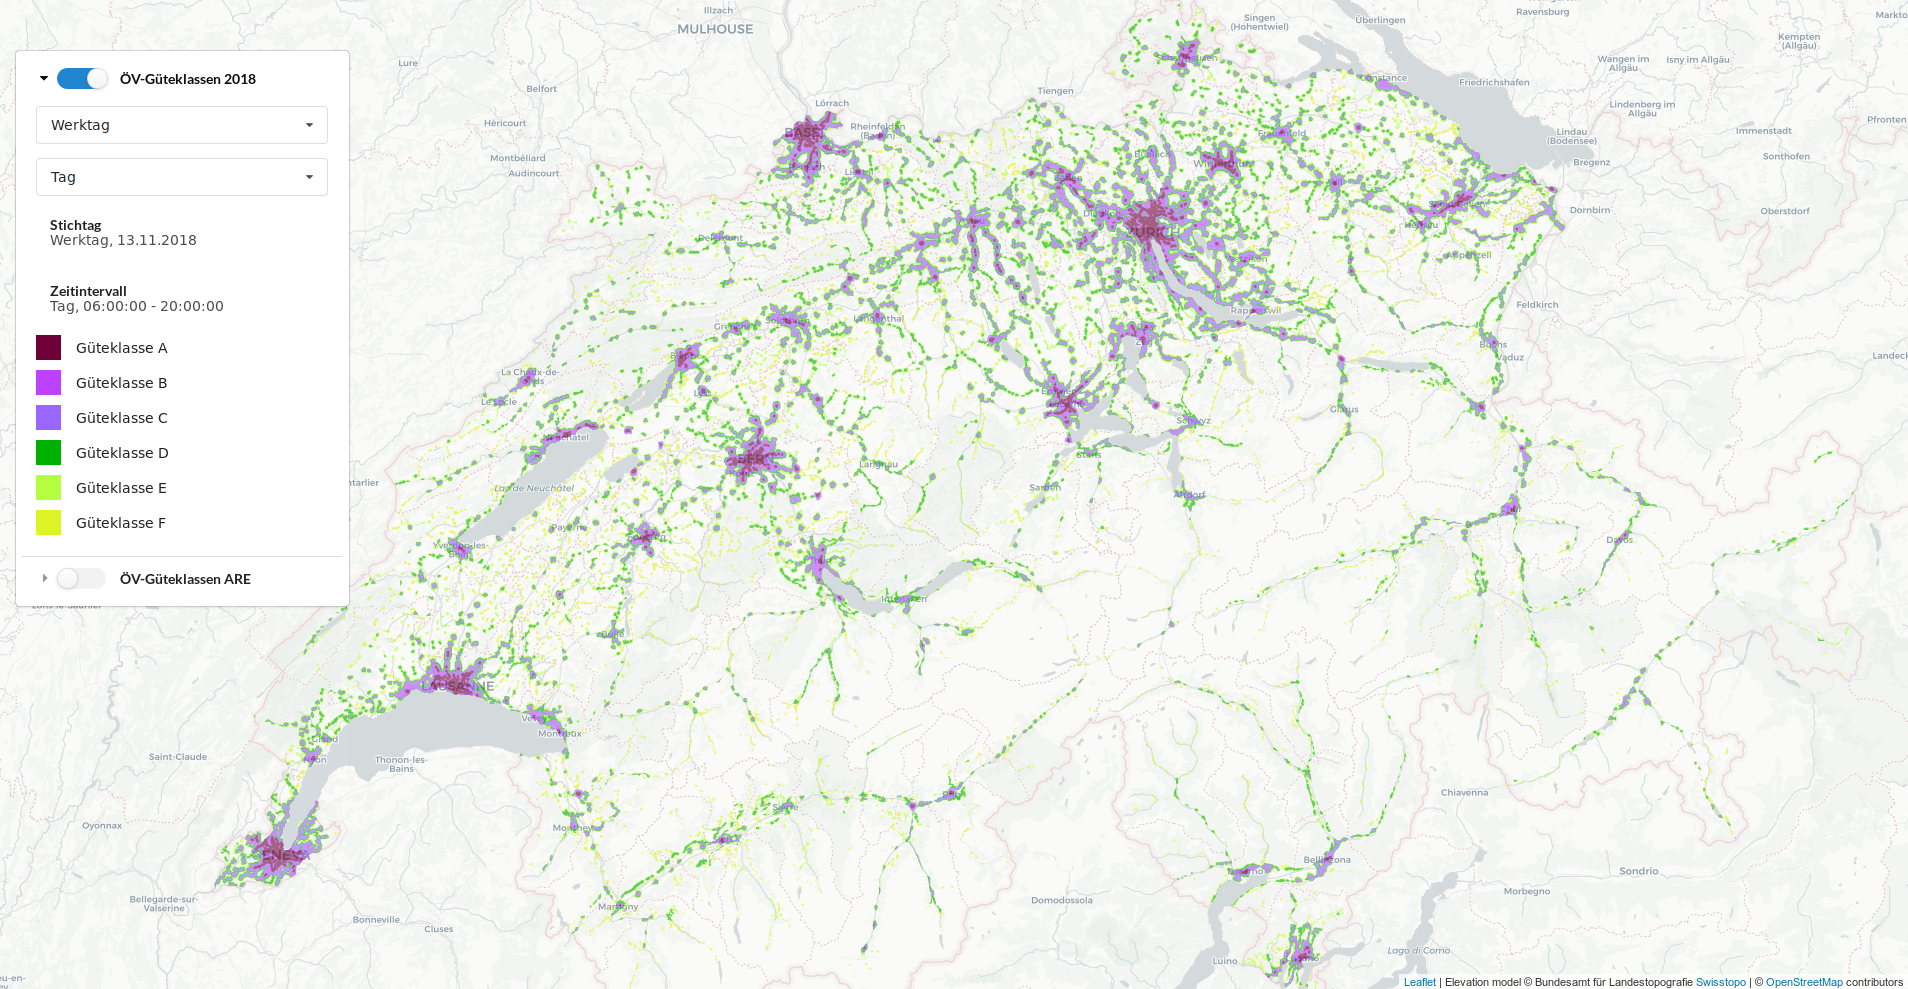
\includegraphics[width=1\linewidth]{technicalreport/img/resultat_oevgk18_uebersicht}
    \caption[Darstellung der berechneten ÖV-Güteklassen in der Web-Applikation]{Darstellung der berechneten ÖV-Güteklassen in der Web-Applikation}
    \label{fig:mntg_sum_resultat_webapp_uebersicht}
\end{figure}

Dabei wird unter anderem zusätzlich die Wegführung berücksichtigt, wie in Abbildung \ref{fig:mgmt_summary_vergleich_wegfuehrung} ersichtlich ist.
Die Topographie wird durch die Verwendung von Leistungskilometern in der Berechnung des Einzugsgebiet miteinbezogen.

\begin{figure}[ht]
    \centering
    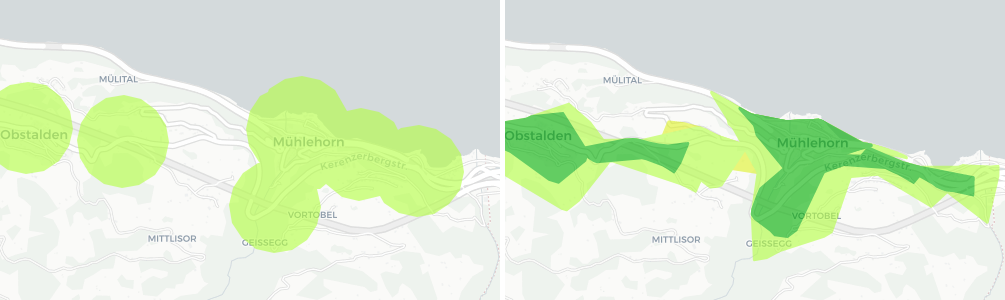
\includegraphics[width=0.8\linewidth]{start/img/vergleich_wegfuehrung}
    \caption[Vergleich zur Einfluss der Wegführung]{Vergleich zur Einfluss der Wegführung. Oben: ÖV-Güteklassen von \ac{ARE}. Unten: ÖV-Güteklassen 2018.}
    \label{fig:mgmt_summary_vergleich_wegfuehrung}
\end{figure}

\paragraph{Ausblick}~\\
In der vorliegenden Arbeit wurde beim Berechnen der Erreichbarkeit der Fokus auf eine routen-basierte Methode, namentlich Isochronen, gelegt.
Ein weiterer spannender Ansatz, welcher in Betracht gezogen werden kann, ist ein grid- beziehungsweise raster-basierter Ansatz.
In Abbildung \ref{fig:mgmt_summary_grid_based_approach} wurde dieser Ansatz für die Berechnung der Reisezeit zu einer Haltestelle eines Fussgängers verwendet.
Dabei wird über ein Gebiet ein Raster gelegt und den Rastern eine Kategorie mit zugehörigen Kosten zugewiesen.
Bei den Kosten handelt es sich im abgebildeten Fall um die Überwindungsgeschwindigkeit des jeweiligen Rasters.
So erhält ein Raster mit einem Hindernis beispielsweise die Geschwindigkeit 0 km/h und eine Grünfläche 2 km/h.
Dies hat unter anderem den Vorteil, dass man nicht direkt vom Routing-Netzwerk abhängig ist und auch offene Flächen wie Plätze und Grünflächen einbezogen werden.

Es lässt sich darüber streiten, ob alle Grünflächen von Fussgänger begehbar sind.
Ebenfalls lassen sich offene Fläche für die bestehende Lösung durch eine Vorverarbeitung des Routing-Netzwerk beispielsweise durch \emph{PlazaRoute}~\cite{plaza_route} ins Routing-Netzwerk integrieren.

\begin{figure}[ht]
    \centering
    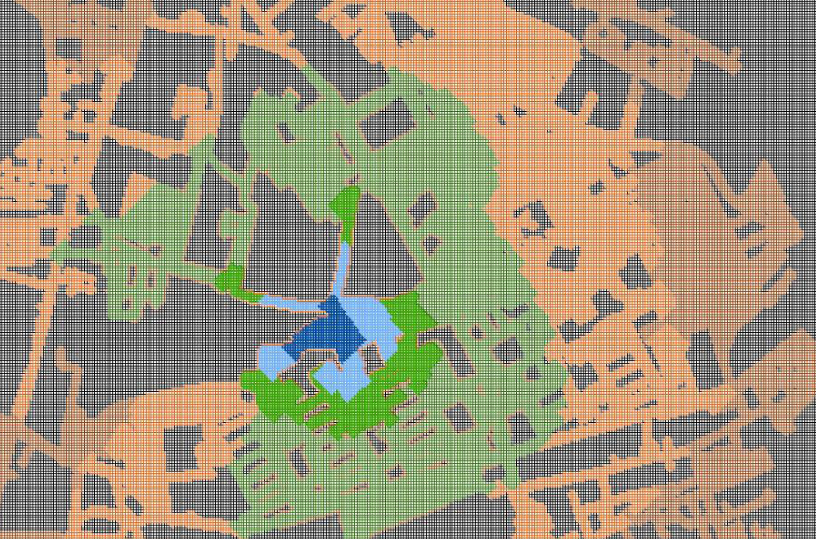
\includegraphics[width=0.6\linewidth]{start/img/grid_based_approach.png}
    \caption[Grid- beziehungsweise raster-basierter Ansatz]{Grid- beziehungsweise raster-basierter Ansatz~\cite{pedestrian_accessibility_planning}}
    \label{fig:mgmt_summary_grid_based_approach}
\end{figure}
